% Tikz picture for the kx-contour at 633 nm

\definecolor{mycolor1}{rgb}{0.92900,0.69400,0.12500}%
\definecolor{mycolor2}{rgb}{0.49400,0.18400,0.55600}%
\definecolor{mycolor3}{rgb}{0.46600,0.67400,0.18800}%
\definecolor{mycolor4}{rgb}{0.30100,0.74500,0.93300}%


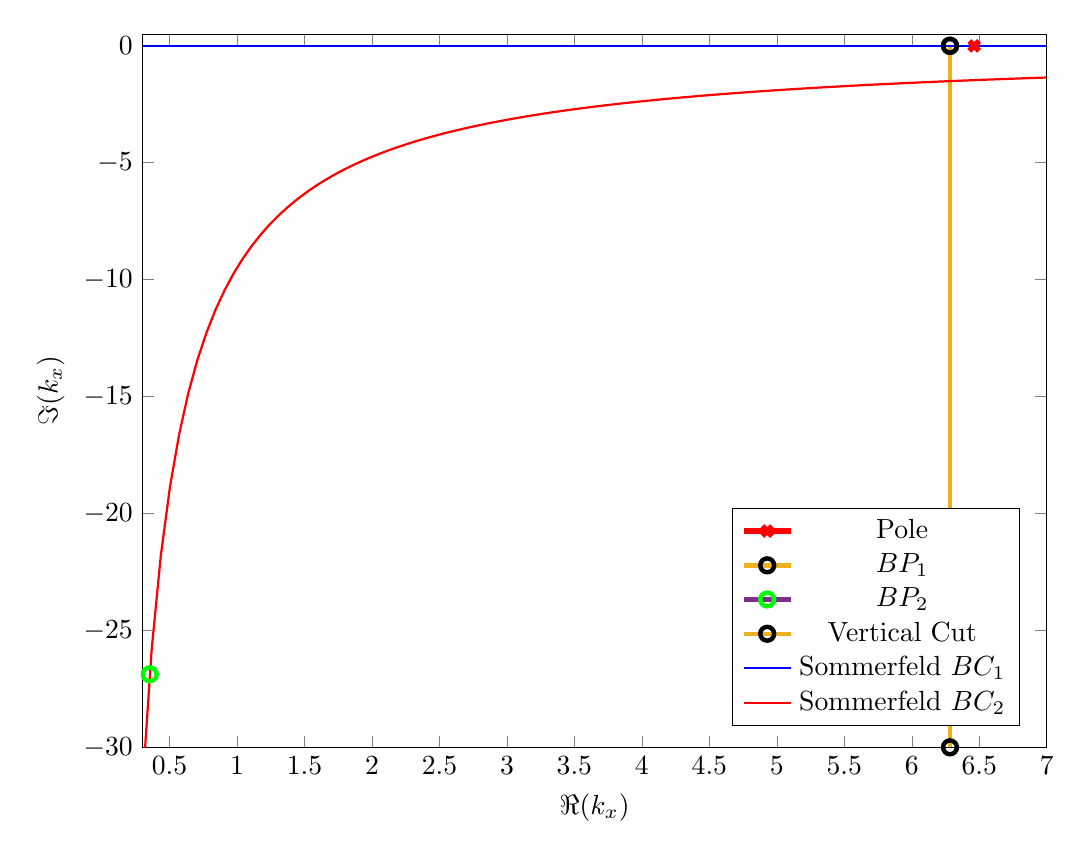
\begin{tikzpicture}
\begin{axis}[domain=0.3:7,  
    width=4.521in,
    height=3.566in,
    at={(0.758in,0.481in)},
    scale only axis,
    unbounded coords=jump,               
    samples=100,
    xlabel=$\Re(k_x)$,
    xmin=.3,
    xmax=7,
    ymin=-30,
    ymax=0.5,
    ylabel=$\Im(k_x)$,
    legend pos=south east]
    \addplot [color=red,solid,line width=2.0pt,mark size=2.5pt,mark=x,mark options={solid,draw=red}]
          table[row sep=crcr]{%
          6.462    -0.005\\
          };
    \addlegendentry{Pole};

     
    \addplot [color=mycolor1,solid,line width=1.6pt,mark size=2.5pt,mark=o,mark options={solid,draw=black}]
          table[row sep=crcr]{%
          6.283   0\\
          };
    \addlegendentry{$BP_1$};  
    
    \addplot [color=mycolor2,solid,line width=1.6pt,mark size=2.5pt,mark=o,mark options={solid,draw=green}]
          table[row sep=crcr]{%
          0.353147222084846   -26.8771717826148\\
          };
    \addlegendentry{$BP_2$};

    \addplot [color=mycolor1,solid,line width=1.6pt,mark size=2.5pt,mark=o,mark options={solid,draw=black}]
          table[row sep=crcr]{%
          6.283   0\\
          6.283   -30\\
          };
    \addlegendentry{Vertical Cut};

    \addplot [color=blue,thick] {0}; \addlegendentry{Sommerfeld $BC_1$}
    
    \addplot [color=red,thick] {-18.98/(2*x)}; \addlegendentry{Sommerfeld $BC_2$};


\end{axis}
\end{tikzpicture}
\end{document}